\section{Overview and Implementation Plan}
The Implementation, Integration and Test phases will follow a \textbf{Bottom-Up} strategy. This approach consists in develop and evaluate the components individually, and then integrate them into a larger system. Working with micro-services, this strategy will be followed starting from the low level components (model, login, and registration) and then continuing building the entire ecosystem around them. At each step some driver will be created in order to test the components. This strategy will allow developers to keep tracks of eventual bugs or errors, and furthermore will allow a parallel developing workflow.

\section{Integration Strategy}
The implementation will be executed in a bottom-up way, starting from the basic feature and component, and after them, with their related test, the above components will be implemented.

\begin{figure}[H]
The implementation starts with the model component and its test.
    \begin{center}
        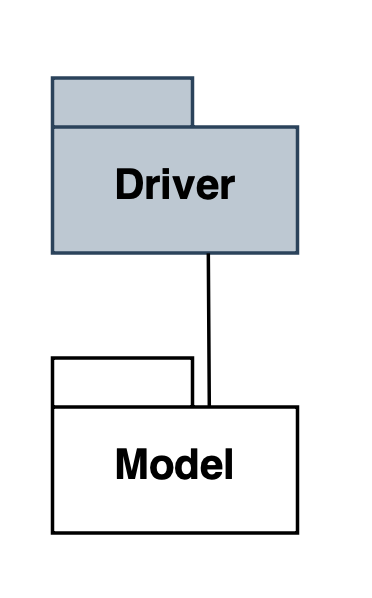
\includegraphics[width=3cm]{images/IntegrationStrategy/model.png}
        \caption{Model implementation}
    \end{center}
\end{figure}

\begin{figure}[H]
The implementation continues with the Login and Signup components, with a particular attention to the university and the Revenue Agency API interaction. At the same time the creation of an Adv of an internship and the Update of a profile can be implemented.\newline
    \begin{center}
        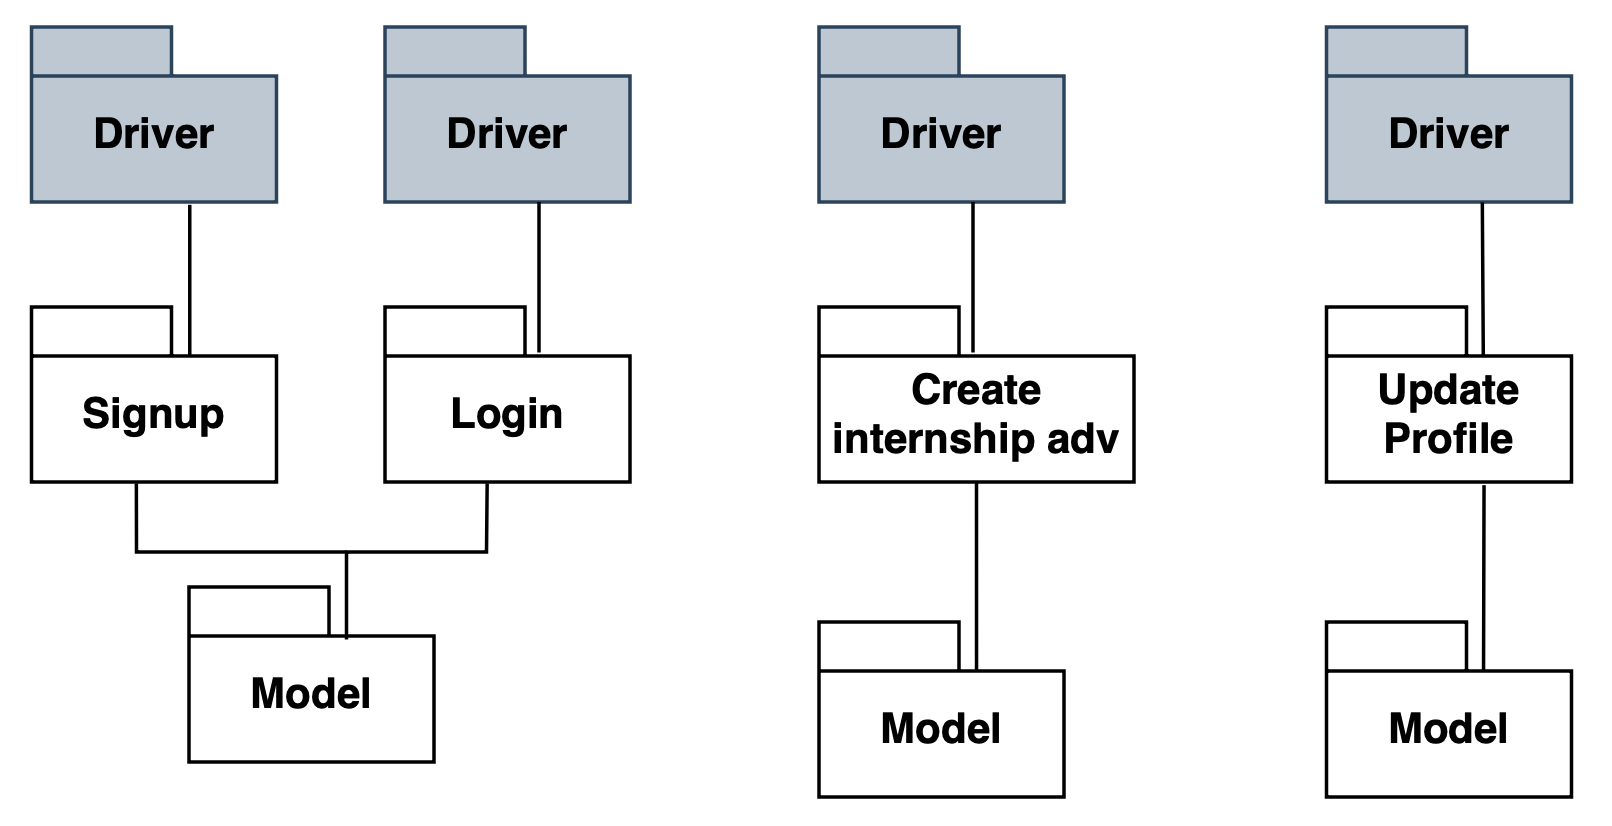
\includegraphics[width=10cm]{images/IntegrationStrategy/login_signup_adv_update.png}
        \caption{Login, Signup, creation of an adv and the update of a profile implementation}
    \end{center}
\end{figure}

\begin{figure}[H]
After Adv creation, Proactive research and Recommendation can be implemented, as long as the creation of the Interview form.\newline
    \begin{center}
        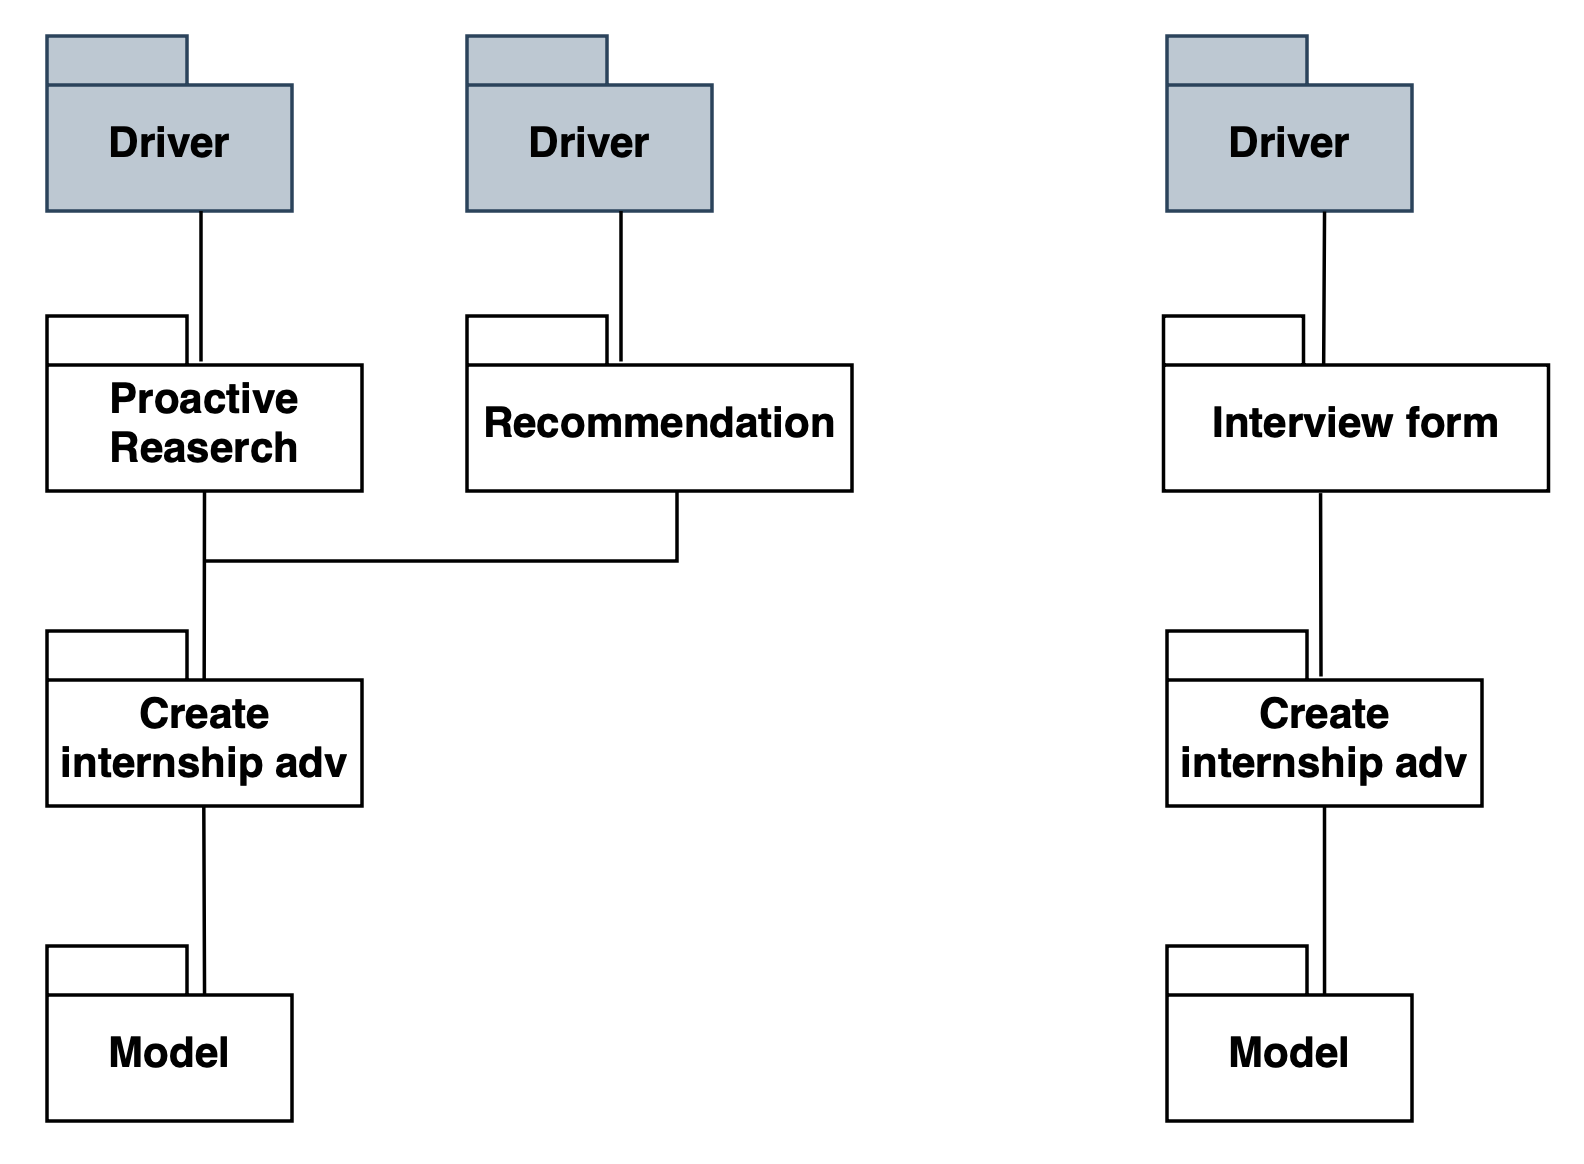
\includegraphics[width=10cm]{images/IntegrationStrategy/proac_recom_intForm.png}
        \caption{Proactive Research, Recommendation and interview form implementation}
    \end{center}
\end{figure}

\begin{figure}[H]
The implementation continues with the Request component, which is directly linked to the Recommendation and to the Proactive Research.
    \begin{center}
        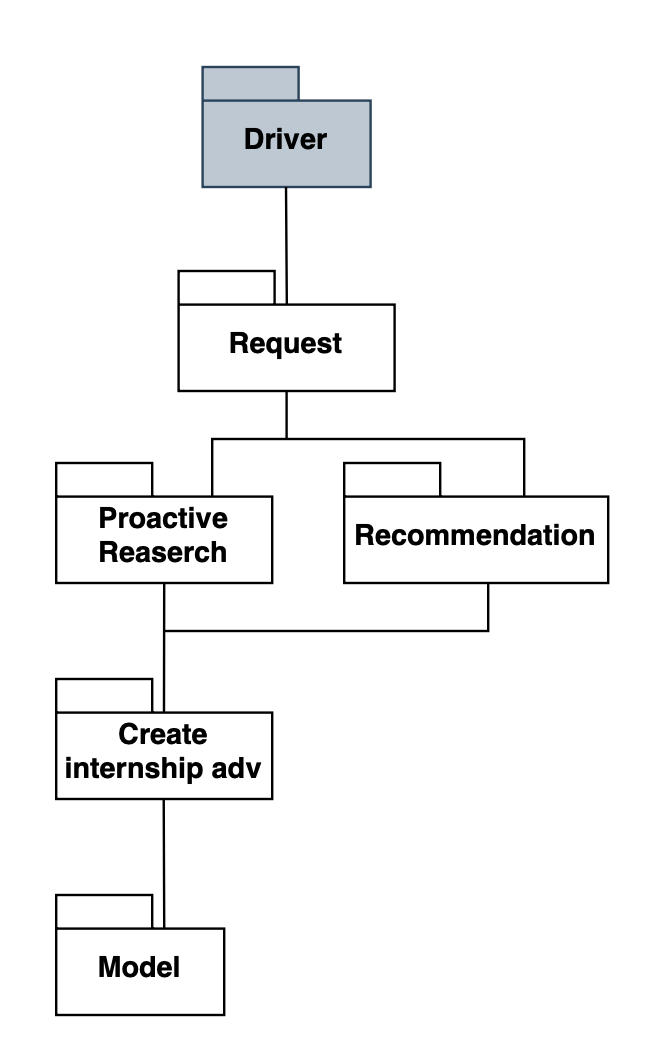
\includegraphics[width=8cm]{images/IntegrationStrategy/req.png}
        \caption{Request implementation}
    \end{center}
\end{figure}

\begin{figure}[H]
After Request implementation, the Match component can be implemented.\newline
    \begin{center}
        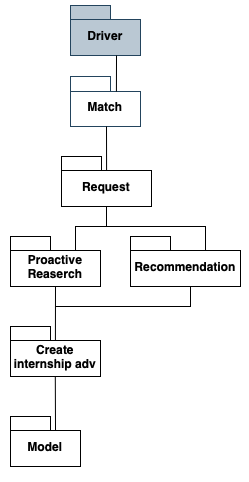
\includegraphics[width=8cm]{images/IntegrationStrategy/match.png}
        \caption{Match and Feedback implementation}
    \end{center}
\end{figure}

\begin{figure}[H]
Then the Interview i implemented and at the same time the Feedback section can be implemented and, during these finals implementation, the system can be joined in order test it in its entirety.
    \begin{center}
        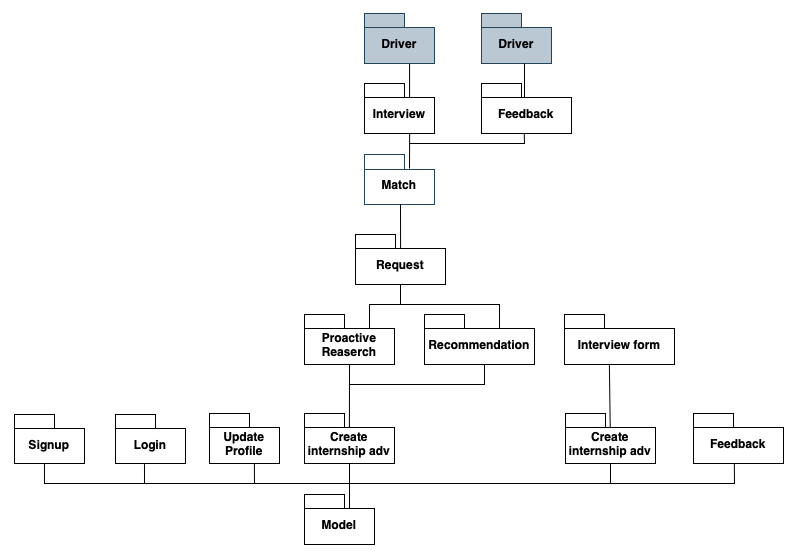
\includegraphics[width=15cm]{images/IntegrationStrategy/interview_feedback.png}
        \caption{Interview and Feedback implementation and join all the system}
    \end{center}
\end{figure}

\begin{figure}[H]
The latter implementation section will involve the Page Manager and all the pages of the Application.
    \begin{center}
        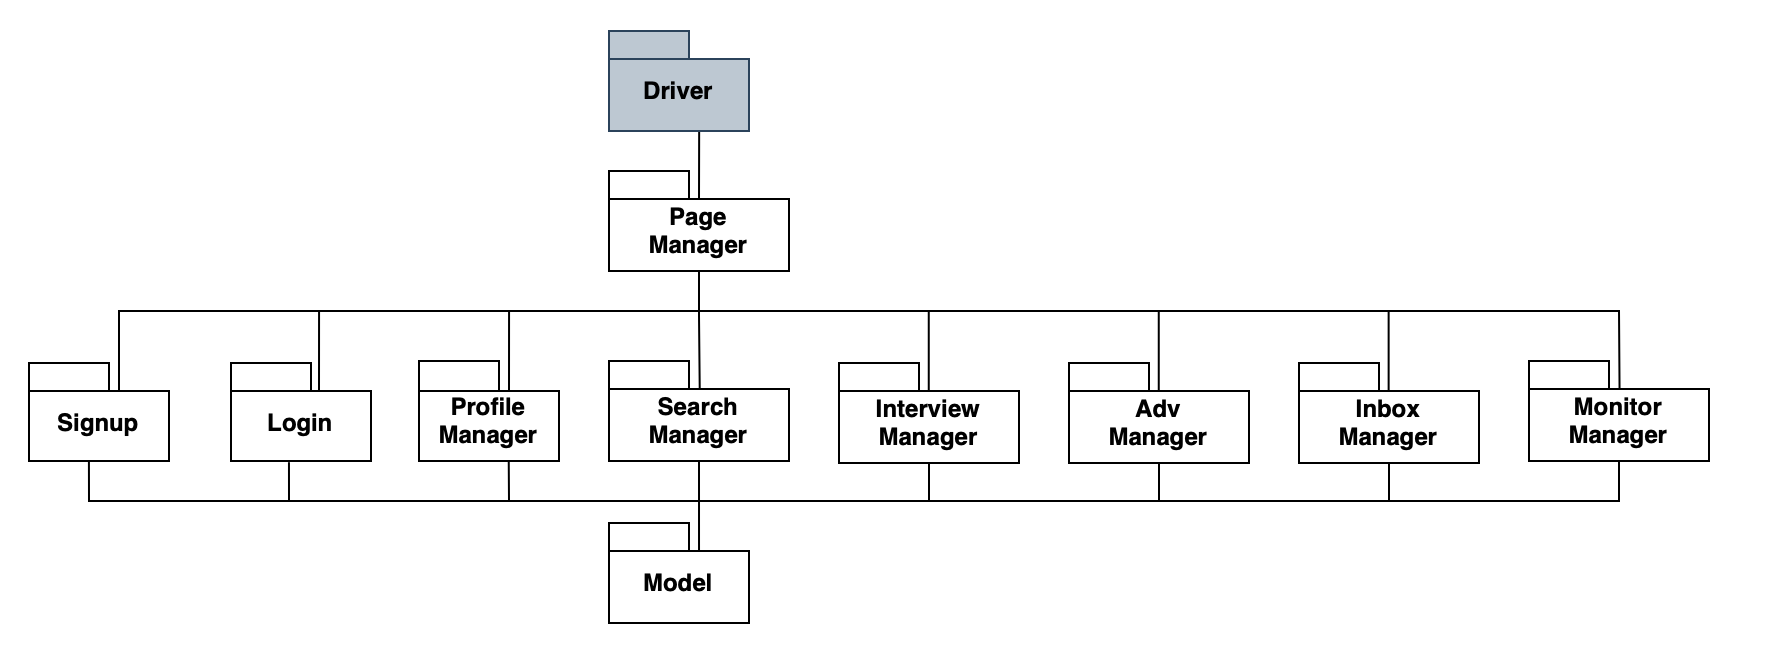
\includegraphics[width=15cm]{images/IntegrationStrategy/page_manager.png}
    \caption{View implementation}
    \end{center}
\end{figure}

\section{System Testing Strategy}
Following the Bottom-Up strategy, every component will be tested with a Driver during the implementation phase but also during the integration phase, in order to assure its functionality independently but also its communication features with all the other components of the system. The test that will be performed are:
\begin{itemize}
    \item \textbf{Functional test:}
    This test sections will ensure that every components fulfill the designated job, accordingly with the system goals, requirement and functionality of the system.
    \item \textbf{Performance test:}
    This type of test are designated to finds bottlenecks and identify some critical situation that may occur during an heavy workload periods. This tests are also useful to get some idea of possible future update and enhancements.
    \item \textbf{Load test:}
    This type of test will cover the discover of memory problems such as leak or overflows.
    \item \textbf{UI test:}
    This type of test will evaluate the Usability of the System for all the users, and will establish if the System works on different type of browser.
\end{itemize}